\documentclass[border=10pt]{standalone}

\usepackage{tikz}
\usepackage{tikzsymbols}
\usetikzlibrary{calc,patterns,shapes.geometric}

\def\centerarc[#1](#2)(#3:#4:#5){\draw[#1] ($(#2)+({#5*cos(#3)},{#5*sin(#3)})$) arc (#3:#4:#5);}

\begin{document}
	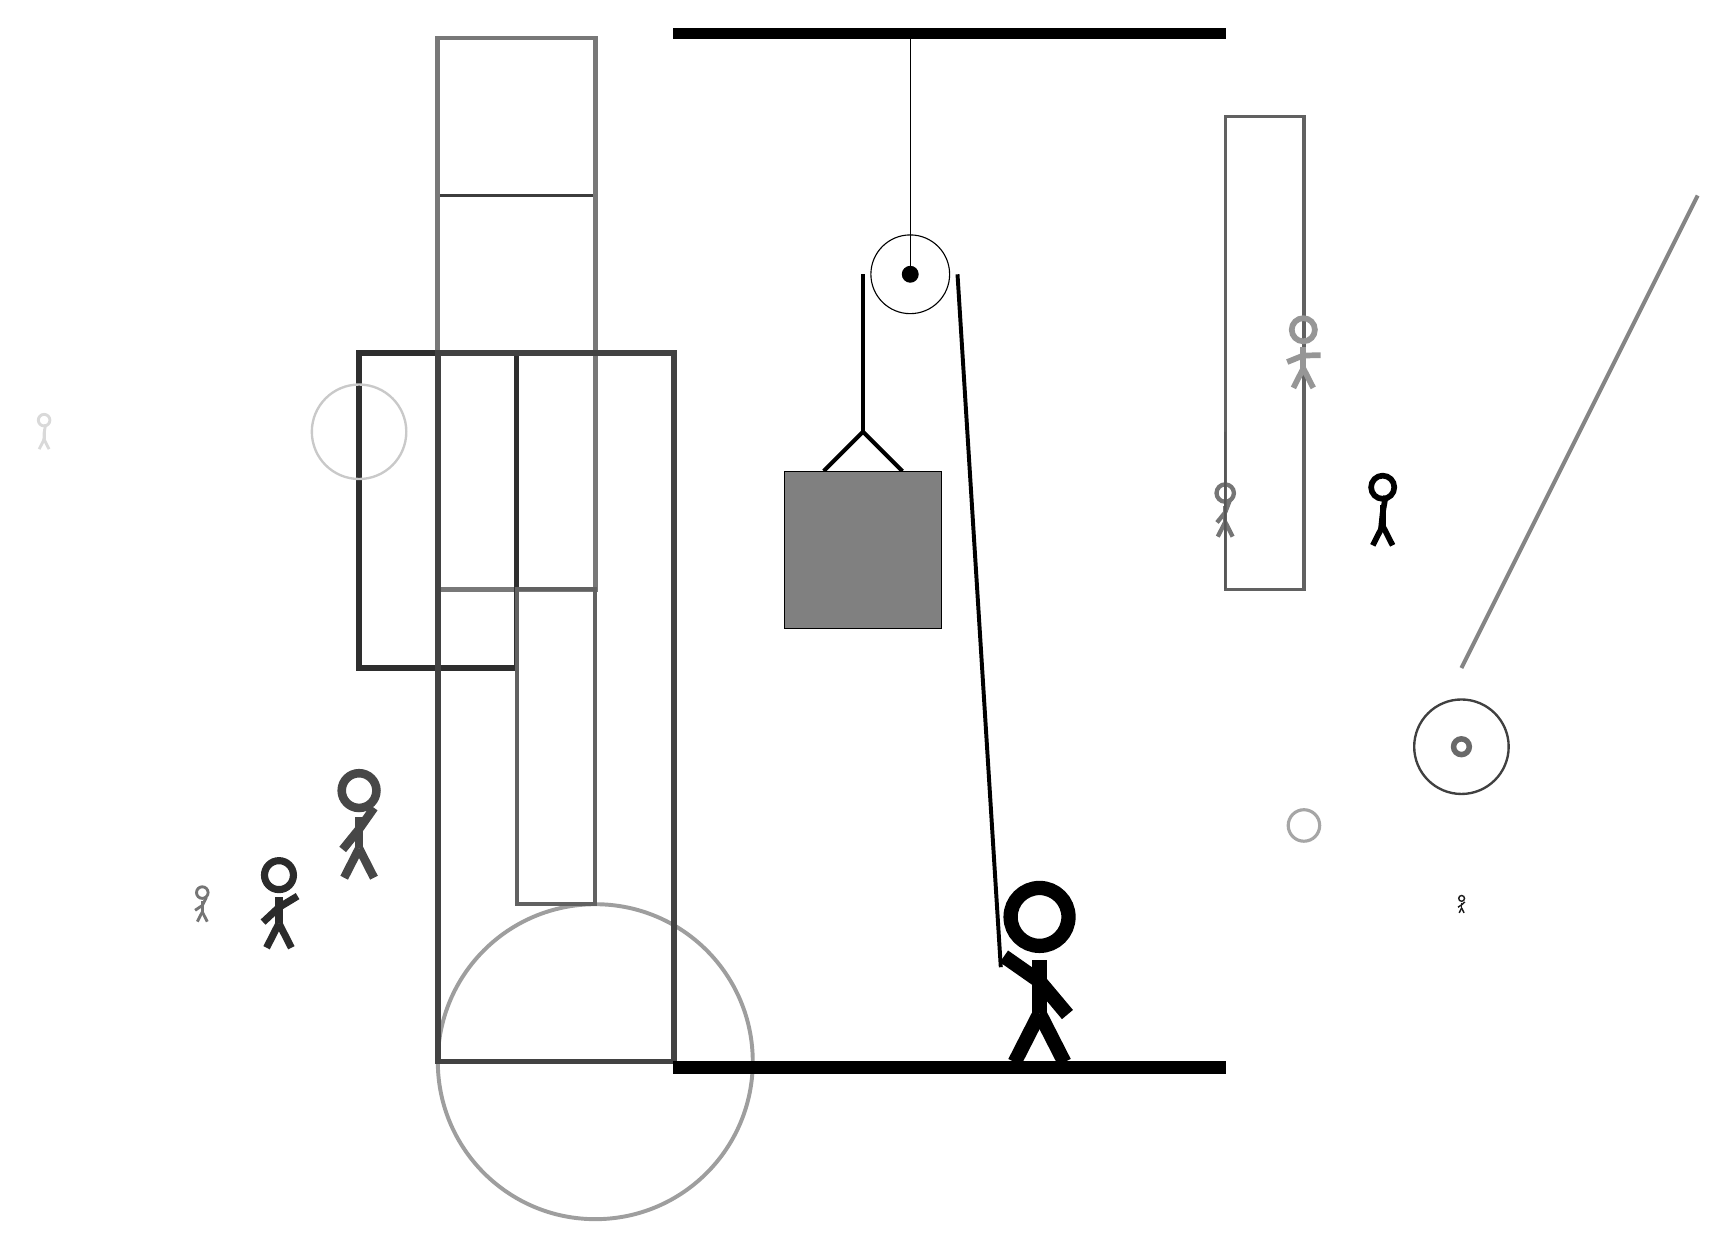
\begin{tikzpicture}
		%%%%% START %%%%%
		
		\draw[fill=black] (-2, 10) rectangle (5, 10.125);
		
		\draw (1, 7) circle (0.5);
		\draw[fill=black] (1, 7) circle (0.1);
		\draw (1, 10) -- (1, 7);
		
		\draw[line width=0.5mm] (-0.1, 4.5) -- (0.4, 5.0) -- (0.9, 4.5);
		\draw[fill=black!50] (-0.6, 4.5) rectangle (1.4, 2.5);
		
		\draw[line width=0.5mm] (0.4, 7) -- (0.4, 5.0);
		\centerarc[line width=0.5mm](1, 7)(0:180:0.6);
		\draw[line width=0.5mm](1.6, 7) -- (2.15, -1.8);
		
		\node[line width=0.6mm, color=black!54] at (-8, -1) {\Strichmaxerl[2][34][63]};
		
		\draw [line width=0.4mm, color=black!35](6, 0) circle (0.2);
		\draw[line width=0.3mm, color=black!76] (-3, 3) rectangle (-5, 8);
		\draw[line width=0.5mm, color=black!58](-6, 2) -- (-5, 2);
		
		\draw[line width=0.6mm, color=black!53] (-3, 3) rectangle (-5, 10);
		\node[line width=0.7mm, color=black!100] at (7, 4) {\Strichmaxerl[4][84][80]};
		\node[line width=0.2mm, color=black!72] at (-6, 0) {\Strichmaxerl[6][51][55]};
		\node[line width=0.2mm, color=black!54] at (5, 4) {\Strichmaxerl[3][51][69]};
		\draw[line width=0.7mm, color=black!82] (-4, 2) rectangle (-6, 6);
		
		\draw [line width=0.3mm, color=black!21](-6, 5) circle (0.6);
		\draw[line width=0.5mm, color=black!48](8, 2) -- (11, 8);
		\draw [line width=0.5mm, color=black!38](-3, -3) circle (2.0);
		\draw[line width=0.5mm, color=black!62] (-3, -1) rectangle (-4, 3);
		
		\draw[line width=0.7mm, color=black!74] (-2, 6) rectangle (-5, -3);
		\node[line width=0.5mm, color=black!15] at (-10, 5) {\Strichmaxerl[2][88][80]};
		\draw[line width=0.4mm, color=black!62] (5, 3) rectangle (6, 9);
		
		\node[line width=0.5mm, color=black!83] at (-7, -1) {\Strichmaxerl[5][43][31]};
		\draw[line width=0.2mm, color=black!66] (5, 5) rectangle (5, 3);
		\node[line width=0.6mm, color=black!89] at (8, -1) {\Strichmaxerl[1][34][42]};
		\draw [line width=0.3mm, color=black!75](8, 1) circle (0.6);
		\draw [line width=0.7mm, color=black!59](8, 1) circle (0.1);
		
		\node[line width=0.2mm, color=black!41] at (6, 6) {\Strichmaxerl[4][22][1]};
		
		\node at (2.6, -1.9) {\Strichmaxerl[10][-35][-50]};
		
		\draw[fill=black] (-2, -3) rectangle (5, -3.15);
		
		%%%%% END %%%%%
	\end{tikzpicture}
\end{document}